% Chapter 1

\chapter{Memory Complexity} % Main chapter title

\label{Chapter7}

In this section we provide a method for applying dimensional reduction of the multidimensional scenario, by grouping significant small subsets of the data and concatenating them after embedding. 


\section{Definition}

We define a generalized ID function by:

\begin{equation}
ID_(\overrightarrow{x_1} , \overrightarrow{x_2} ; S) = [ ID(\overrightarrow{x_1}_[S_1],\overrightarrow{x_2}_[S_1]) , \dots , \dots , ID(\overrightarrow{x_1}_[S_g],\overrightarrow{x_2}_[S_g])  ]
\end{equation}

where $S$ is the defined sub-domain group: \\ 

$\{S_i\}_{i=1}^g \qquad,\qquad S_i\subseteq [1, \dots , n] \qquad , \qquad g \in [1, \dots , n]$ \\ 

Where $g$ represents a sub domain which extracts valid demandable information to the user. \\ 

For example when applying ID embedding on \textbf{SIFT[]} descriptors, a certain user may involve only neighbor pairs, where another one may involve just bin-to-bin pairs.

\subsection{SIFT Example}

when applying ID on SIFT [] descriptors (for template matching),  n is 128, which causes time and memory complexity to be scaled by 1282=16384. 
If one user desires, and physically ables to reduce this coefficient, we developed the following generalization.

\begin{figure} \label{s1}
	    \centering
		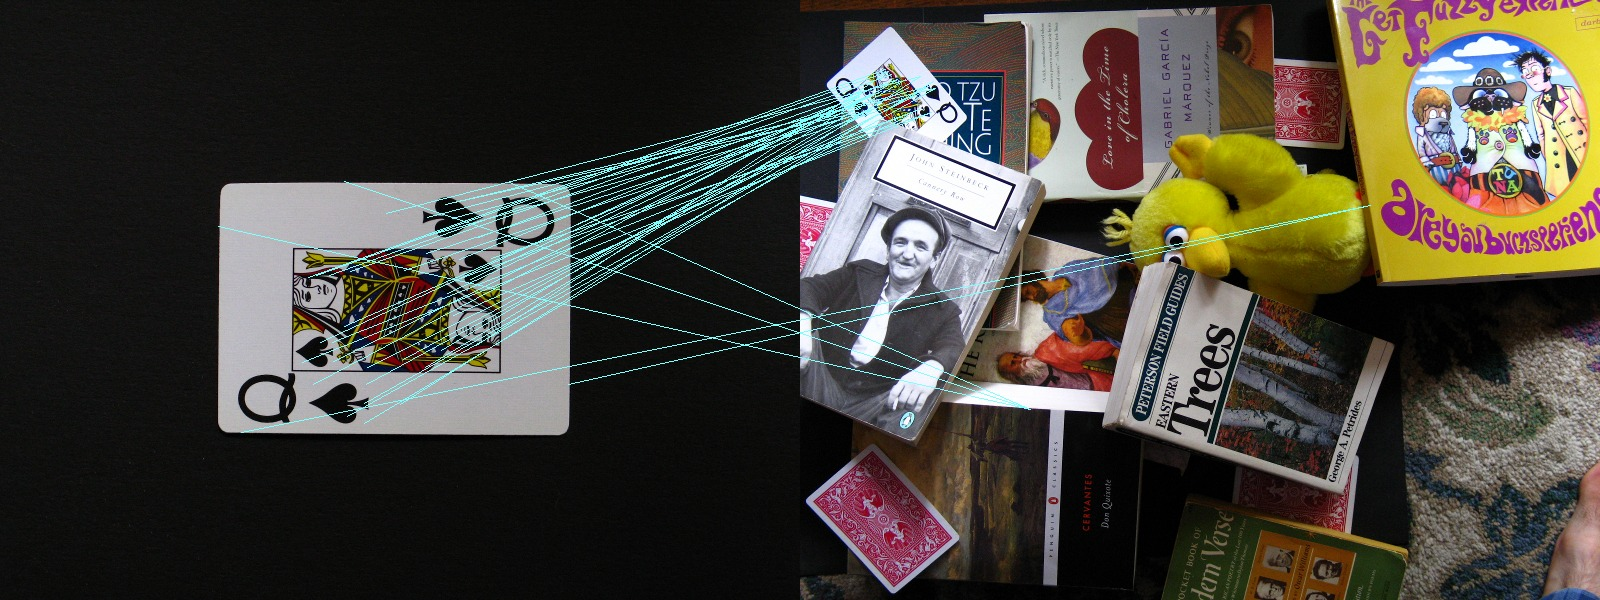
\includegraphics[width=\linewidth,height=12cm,keepaspectratio]{Figures/sift1}
		\caption[SIFT algorithm used for template matching]
		{SIFT algorithm used for template matching. In this example each image is scanned and a set of keypoints (a significant point) is found, and for each keypoints a 3D features vector is calculated. These vectors are being compared between the images, and a similarity is measured among those sets. Here we see that there is a match between both Queen cards in both images, although there are size, orientation, and clearance differences}
\end{figure}
	
\begin{figure} \label{s2}
		\centering
		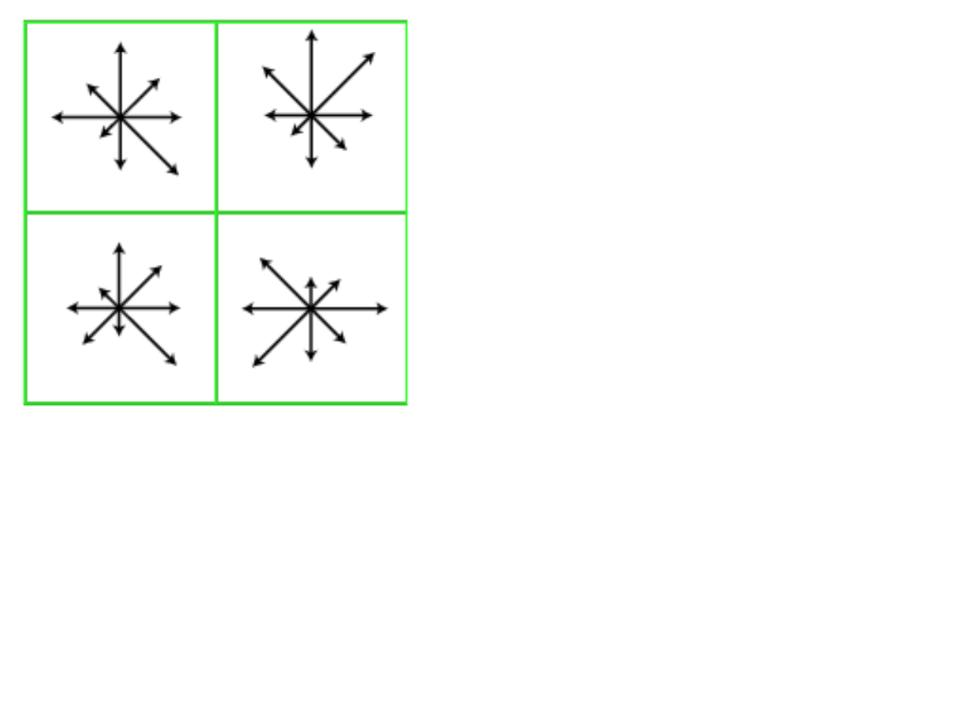
\includegraphics[width=12cm,height=12cm,keepaspectratio]{Figures/sift2}
		\caption[SIFT kp descriptor example]
		{SIFT keypoint descriptor scheme. A 16x16 neighborhood around the keypoint is taken. It is divided into 16 sub-blocks of 4x4 size. For each sub-block, 8 bin orientation histogram is created. So a total of 128 bin values are available. It is represented as a vector to form keypoint descriptor. In addition to this, several measures are taken to achieve robustness against illumination changes, rotation etc.}
\end{figure}

